
\documentclass[a4paper,11pt]{article}
\usepackage[a4paper, margin=8em]{geometry}

% usa i pacchetti per la scrittura in italiano
\usepackage[french,italian]{babel}
\usepackage[T1]{fontenc}
\usepackage[utf8]{inputenc}
\frenchspacing 

% usa i pacchetti per la formattazione matematica
\usepackage{amsmath, amssymb, amsthm, amsfonts}

% usa altri pacchetti
\usepackage{gensymb}
\usepackage{hyperref}
\usepackage{standalone}

% imposta il titolo
\title{Appunti Comunicazioni Numeriche}
\author{Luca Seggiani}
\date{2026}

% imposta lo stile
% usa helvetica
\usepackage[scaled]{helvet}
% usa palatino
\usepackage{palatino}
% usa un font monospazio guardabile
\usepackage{lmodern}

\renewcommand{\rmdefault}{ppl}
\renewcommand{\sfdefault}{phv}
\renewcommand{\ttdefault}{lmtt}

% disponi il titolo
\makeatletter
\renewcommand{\maketitle} {
	\begin{center} 
		\begin{minipage}[t]{.8\textwidth}
			\textsf{\huge\bfseries \@title} 
		\end{minipage}%
		\begin{minipage}[t]{.2\textwidth}
			\raggedleft \vspace{-1.65em}
			\textsf{\small \@author} \vfill
			\textsf{\small \@date}
		\end{minipage}
		\par
	\end{center}

	\thispagestyle{empty}
	\pagestyle{fancy}
}
\makeatother

% disponi teoremi
\usepackage{tcolorbox}
\newtcolorbox[auto counter, number within=section]{theorem}[2][]{%
	colback=blue!10, 
	colframe=blue!40!black, 
	sharp corners=northwest,
	fonttitle=\sffamily\bfseries, 
	title=~\thetcbcounter: #2, 
	#1
}

% disponi definizioni
\newtcolorbox[auto counter, number within=section]{definition}[2][]{%
	colback=red!10,
	colframe=red!40!black,
	sharp corners=northwest,
	fonttitle=\sffamily\bfseries,
	title=~\thetcbcounter: #2,
	#1
}

% U.D.M
\newcommand{\amp}{\ensuremath{\mathrm{A}}}
\newcommand{\volt}{\ensuremath{\mathrm{V}}}
\newcommand{\meter}{\ensuremath{\mathrm{m}}}
\newcommand{\second}{\ensuremath{\mathrm{s}}}
\newcommand{\farad}{\ensuremath{\mathrm{F}}}
\newcommand{\henry}{\ensuremath{\mathrm{H}}}
\newcommand{\siemens}{\ensuremath{\mathrm{S}}}

% circuiti
\usepackage{circuitikz}
\usetikzlibrary{babel}

% disegni
\usepackage{pgfplots}
\pgfplotsset{width=10cm,compat=1.9}

% disponi codice
\usepackage{listings}
\usepackage[table]{xcolor}

\lstdefinestyle{codestyle}{
		backgroundcolor=\color{black!5}, 
		commentstyle=\color{codegreen},
		keywordstyle=\bfseries\color{magenta},
		numberstyle=\sffamily\tiny\color{black!60},
		stringstyle=\color{green!50!black},
		basicstyle=\ttfamily\footnotesize,
		breakatwhitespace=false,         
		breaklines=true,                 
		captionpos=b,                    
		keepspaces=true,                 
		numbers=left,                    
		numbersep=5pt,                  
		showspaces=false,                
		showstringspaces=false,
		showtabs=false,                  
		tabsize=2
}

\lstdefinestyle{shellstyle}{
		backgroundcolor=\color{black!5}, 
		basicstyle=\ttfamily\footnotesize\color{black}, 
		commentstyle=\color{black}, 
		keywordstyle=\color{black},
		numberstyle=\color{black!5},
		stringstyle=\color{black}, 
		showspaces=false,
		showstringspaces=false, 
		showtabs=false, 
		tabsize=2, 
		numbers=none, 
		breaklines=true
}

\lstdefinelanguage{javascript}{
	keywords={typeof, new, true, false, catch, function, return, null, catch, switch, var, if, in, while, do, else, case, break},
	keywordstyle=\color{blue}\bfseries,
	ndkeywords={class, export, boolean, throw, implements, import, this},
	ndkeywordstyle=\color{darkgray}\bfseries,
	identifierstyle=\color{black},
	sensitive=false,
	comment=[l]{//},
	morecomment=[s]{/*}{*/},
	commentstyle=\color{purple}\ttfamily,
	stringstyle=\color{red}\ttfamily,
	morestring=[b]',
	morestring=[b]"
}

% disponi sezioni
\usepackage{titlesec}

\titleformat{\section}
	{\sffamily\Large\bfseries} 
	{\thesection}{1em}{} 
\titleformat{\subsection}
	{\sffamily\large\bfseries}   
	{\thesubsection}{1em}{} 
\titleformat{\subsubsection}
	{\sffamily\normalsize\bfseries} 
	{\thesubsubsection}{1em}{}

% disponi alberi
\usepackage{forest}

\forestset{
	rectstyle/.style={
		for tree={rectangle,draw,font=\large\sffamily}
	},
	roundstyle/.style={
		for tree={circle,draw,font=\large}
	}
}

% disponi algoritmi
\usepackage{algorithm}
\usepackage{algorithmic}
\makeatletter
\renewcommand{\ALG@name}{Algoritmo}
\makeatother

% disponi numeri di pagina
\usepackage{fancyhdr}
\fancyhf{} 
\fancyfoot[L]{\sffamily{\thepage}}

\makeatletter
\fancyhead[L]{\raisebox{1ex}[0pt][0pt]{\sffamily{\@title \ \@date}}} 
\fancyhead[R]{\raisebox{1ex}[0pt][0pt]{\sffamily{\@author}}}
\makeatother

\begin{document}
% sezione (data)
\section{Lezione del 19-05-26}

% stili pagina
\thispagestyle{empty}
\pagestyle{fancy}

% testo
\subsection{Sistemi di comunicazione in banda base}
I sistemi di comunicazione in \textit{banda base} sono quelli dove il segnale non viene modulato a frequenza portante, ma trasmesso demodulato (cioè nella banda base).

In particolare, ci interessiamo ai sistemi di comunicazione \textbf{PAM} (\textit{Pulse Amplitude Modulation}) in banda base, cioè basati sulla codifica dei valori numerici in costellazioni simmetriche. Queste possono essere binarie, quaternarie, ottnoarie, ecc... e simmetriche rispetto allo 0.

Chiaramente, avevamo detto che al crescere della dimensione $Q$ delle parole codificate dai simboli PAM, la probabilità di errore (cioè il numero di simboli da distinguere aumenta). 

Segue la mappa un \textit{filtro} di interpolazione, solitamente di tipo $\mathrm{rect}$, che riporta i simboli ottenuti (interpretati come ampiezze di impulsi rettangolari in PAM) nel dominio analogico.

\par\smallskip

Come avevamo visto alla scorsa lezione, non possiamo trattare il segnale in ingresso come deterministico, ma dobbiamo assumerlo come aleatorio e considerare le densità spettrali di potenza. In particolare, la densità spettrale sarà:
$$
S_S(f) = \frac{1}{T_S} S_\alpha(f) | G_T(f) |^2
$$
cioè la densità spettrale dei simboli:
$$
S_\alpha(f) = \sum_m R_\alpha(m) e^{-i 2 \pi m f T_S}
$$
per la risposta del filtro di interpolazione. Resta da calcolare la funzione di autocorrelazione $R_\alpha(m)$ dei simboli in uscita dal mappatore, che abbiamo dalla scorsa lezione:
$$
R_a(m) =
\begin{cases}
	E\{a_i^2\}, \quad m = 0 \\
	0, \quad m \neq 0
\end{cases}
= E \{ a_i^2 \} \delta(m) = \sigma_a^2 \delta(m)
$$
cioè la delta per il valore quadratico medio. Notiamo che il valore quadratico medio è pari al quadrato della varianza, in quanto la media per costellazioni simmetriche è nulla, e quindi:
$$
\sigma_a^2 = E \{ a_i^2 \} = \frac{(\# M)^2 - 1}{3}
$$

Segue che in in sistema PAM con alfabeto $M$:
$$
S_\alpha(f) = \sigma_a^2 = \frac{(\# M)^2 - 1}{3}
$$
e la densità spettrale di potenza del segnale è pari a:
$$
S_S(f) = \frac{1}{T_S} \frac{(\# M)^2 - 1}{3} | G_T(f) |^2
$$
Gli unici parametri significativi in questa equazione sono la dimensione dell'alfabeto $\# M$ (cioè $2^Q$ sui $Q$ bit che l'alfabeto codifica) e la densità di potenza del filtro $G_T(f)$.

\subsubsection{Considerazioni di potenza}
Vogliamo estrarre informazioni sulla potenza complesiva del segnale dalle formule per la densità spettrale di potenza del segnale. Di base la potenza sarà l'integrale della densità:
$$
P_S = \int_{-\infty}^{\infty} S_S(f) \, df = \frac{\sigma_a^2}{T_S} E_{g_T} 
$$
dove $E_{g_T}$ è l0energia complessiva del filtro di interpolazione. A questo punto l'energia impiegata a trasmettere una parola sarà:
$$
E_S = P_S T_S = \sigma_a^2 E_{g_T} 
$$

Come abbiamo visto ampiamente nella scorsa lezione, queste considerazioni si estendono in cascata a tutti gli stadi precedenti al mapppatore e all'interpolatore (cioè al modulatore in banda base). Ad esempio, si ha l'energia sul bit codificato $\{d_n\}$:
$$
E_d = \frac{E_s}{Q} = \frac{1}{\log_2 (\# M)} \frac{(\# M)^2 - 1}{3} E_{g_T}
$$
e, assumendo la codifica identità al codificatore di sorgente, si ha l'energia sul bit trasmesso $\{b_n\}$:
$$
E_b = \frac{1}{r} E_d =  \frac{1}{r} \frac{1}{\log_2 (\# M)} \frac{(\# M)^2 - 1}{3} E_{g_T}
$$

\subsubsection{Considerazioni di banda}
Oltre alle perdite energetiche, vogliamo sapere come impieghiamo la banda disponibile nel sistema di cmounicazione. In particolare, \textit{in banda base}, si ha:
$$
B_s = \frac{1}{2 T_s} = \frac{1}{\log_2(\# M)} \frac{1}{2 T_d} = \frac{1}{r} \frac{1}{\log_2(\# M)} \frac{1}{2 T_b}
$$
dove:
\begin{itemize}
	\item $T_b$ è il perido del bit in uscita dal codificatore si sorgente, che prendiamo fisso; 
	\item $r$ è il rate del codice: diminuendolo (e quindi portando meno bit dati per bit totali) si aumenta la banda usata;
	\item $\log_2(\# M)$ indica la dimensione dell'alfabeto: aumentandola, la si diminuisce la banda usata.
\end{itemize}

\subsection{Ricevitori di sistemi di comunicazione}
Nella lezione 4 avevamo visto la legge di Friis per il rapporto fra potenza ricevuta e potenza trasmessa attraverso antenne (cioè l'\textit{attenuazione}):
$$
\beta = \frac{P_r}{P_t} = \frac{\lambda^2}{(4 \pi d)^2}
$$

Quindi, visto che il rumore veniva modellizzato come termico e costante data la banda:
$$
Pn = B k_B T
$$
avevamo visto anche la seguente espressione per l'\textbf{SNR} (\textit{Signal to Noise Ratio}):
$$
\mathrm{SNR} = P_t \frac{\lambda^2}{(4 \pi d)^2} \frac{1}{B k_B T}
$$

Infine, nella prima lezione avevamo visto l'equazione (dovuta a Shannon) per la capacità di un qualsiasi sistema di comunicazione:
$$
C = B \log_2(1 + \mathrm{SNR}) \, \mathrm{bit/s/Hz}
$$

\subsubsection{Considerazioni di potenza}
Vogliamo riportare queste equazioni al modello visto finora per ottenere una descrizione del \textit{ricevitore} di un dato sistema di comunicazione. Partiamo dal segnale trasmesso in banda base ($S_T(t)$), troviamo il segnale ricevuto (in tempo e densità spettrale):
$$
r(t) = \sqrt{\beta} S_T(t), quad S_r(f) = \beta S_S(f)
$$

La potenza ricevuta complessiva, a questo punto, sarà:
$$
P_r \int_{-\infty}^\infty S_r(f) \, df = \beta P_S
$$

\subsubsection{Ritardo}
Finora abbiamo trascurato il fatto che la trasmissione attraverso il mezzo introduce un \textit{ritardo} $r$ nel segnale ricevuto:
$$
r(t) = \sqrt{\beta} S_R (t - \tau)
$$
dove $r$ si ottiene come:
$$
\tau = \frac{d}{c}
$$
con $d$ distanza fra trasmettitore e ricevitore e $c$ velocità della luce.

Cioè che desideremo dal ritardo sarà che questo sia comparabile col tempo di segnalazione dei simboli (il $T_S$). Prendiamo la $\mathrm{rect}$ in banda base, per cui vale:
$$
B_S = \frac{1}{T_S} = \frac{R_b}{r \log_2(\# M)}
$$
in tal caso vogliamo che, ricavato $T_S$, valga $\tau << T_S$.

\subsubsection{Rumore}
L'ultimo elemento che non abbiamo considerato è il \textit{rumore} (solitamente termico) introdotto dal mezzo in fase di trasmissione. La formula completa sarà:
$$
r(t) = \sqrt{\beta} S_T(t - \tau) + w(t)
$$

La $w(t)$ (che rappresenterà il rumore) sarà stocastica, e potrà essere rappresentata come un processo aleatorio.

\subsubsection{Rappresentazione come filtro}
Ci rendiamo adesso conto che il mezzo (trascurando il rumore) può essere rappresentato come un filtro non distorcente, con risposta in dominio tempo:
$$
h(t) = \sqrt{\beta} \delta(t - \tau)
$$

Data questa definizione, il segnale ricevuto $r(t)$ può essere espresso anche come:
$$
r(t) = S_R(t) \circledast h(t)
$$

A questo punto reintroduciamo il rumore come puramente additivo (\textbf{AWGN}, \textit{Additive Gaussian White Noise}), rappresentato dal rumore gaussiano bianco $w(t)$:
$$
r(t) = S_R(t) \circledast h(t) + w(t)
$$
Dal fatto che il rumore è gaussiano bianco, abbiamo:
$$
w(t) \sim \text{Gaussiano} \implies S_w(f) = \frac{N_0}{2} \sim \frac{k_B T_A}{2}
$$
dove $T_A$ è il \textit{tempo equivalente dell'antenna}.

\subsubsection{Propagazione multipath}
Un'altra caratteristica dei sistemi di comunicazione su mezzo wireless che non abbiamo considerato è quella della propagazione per più \textit{percorsi} che si ha, a causa della riflessione del segnale sugli ostacoli incontrati lungo la strada.

Avremo quindi che, in generale, il segnale ricevuto da un antenna sarà una combinazione lineare di segnali attenuati $\beta_i$ e ritardati $\tau_i$ con valori diversi, ovvero:
$$
r(t) = \sum_i \sqrt{\beta_i} S_T(t - \tau_i) + w(t)
$$

\par\smallskip

Possiamo trascurare gli effetti cumulati del multipath, e prendere il canale come un semplice filtro non distorcente (trascurando il rumore), assumendo che tutti i segnali multipath siano sostanzialmente uguali, e quindi:
$$
r(t) = c(t) + w(t), \quad c(t) = \sum_i \sqrt{\beta} \delta(t - \tau) = A \delta(t - \tau)
$$

Questa ipotesi è comunque valida se i $\tau_i$ sono abbastanza simili fra lori, e si può prendere la somma delle attenuazioni dei segnali in arrivo come:
$$
A = \sum_i \beta_i
$$

\subsection{Struttura del demodulatore}
Dopo aver studiato la struttura del segnale analogico trasformato dal mezzo di trasmissione, vediamo come il demodulatore riporta tale segnale in una serie di parole corrispondenti (sperabilmente) a quelle codificate dal codificatore di canale, al trasmettitore.

\begin{center}
	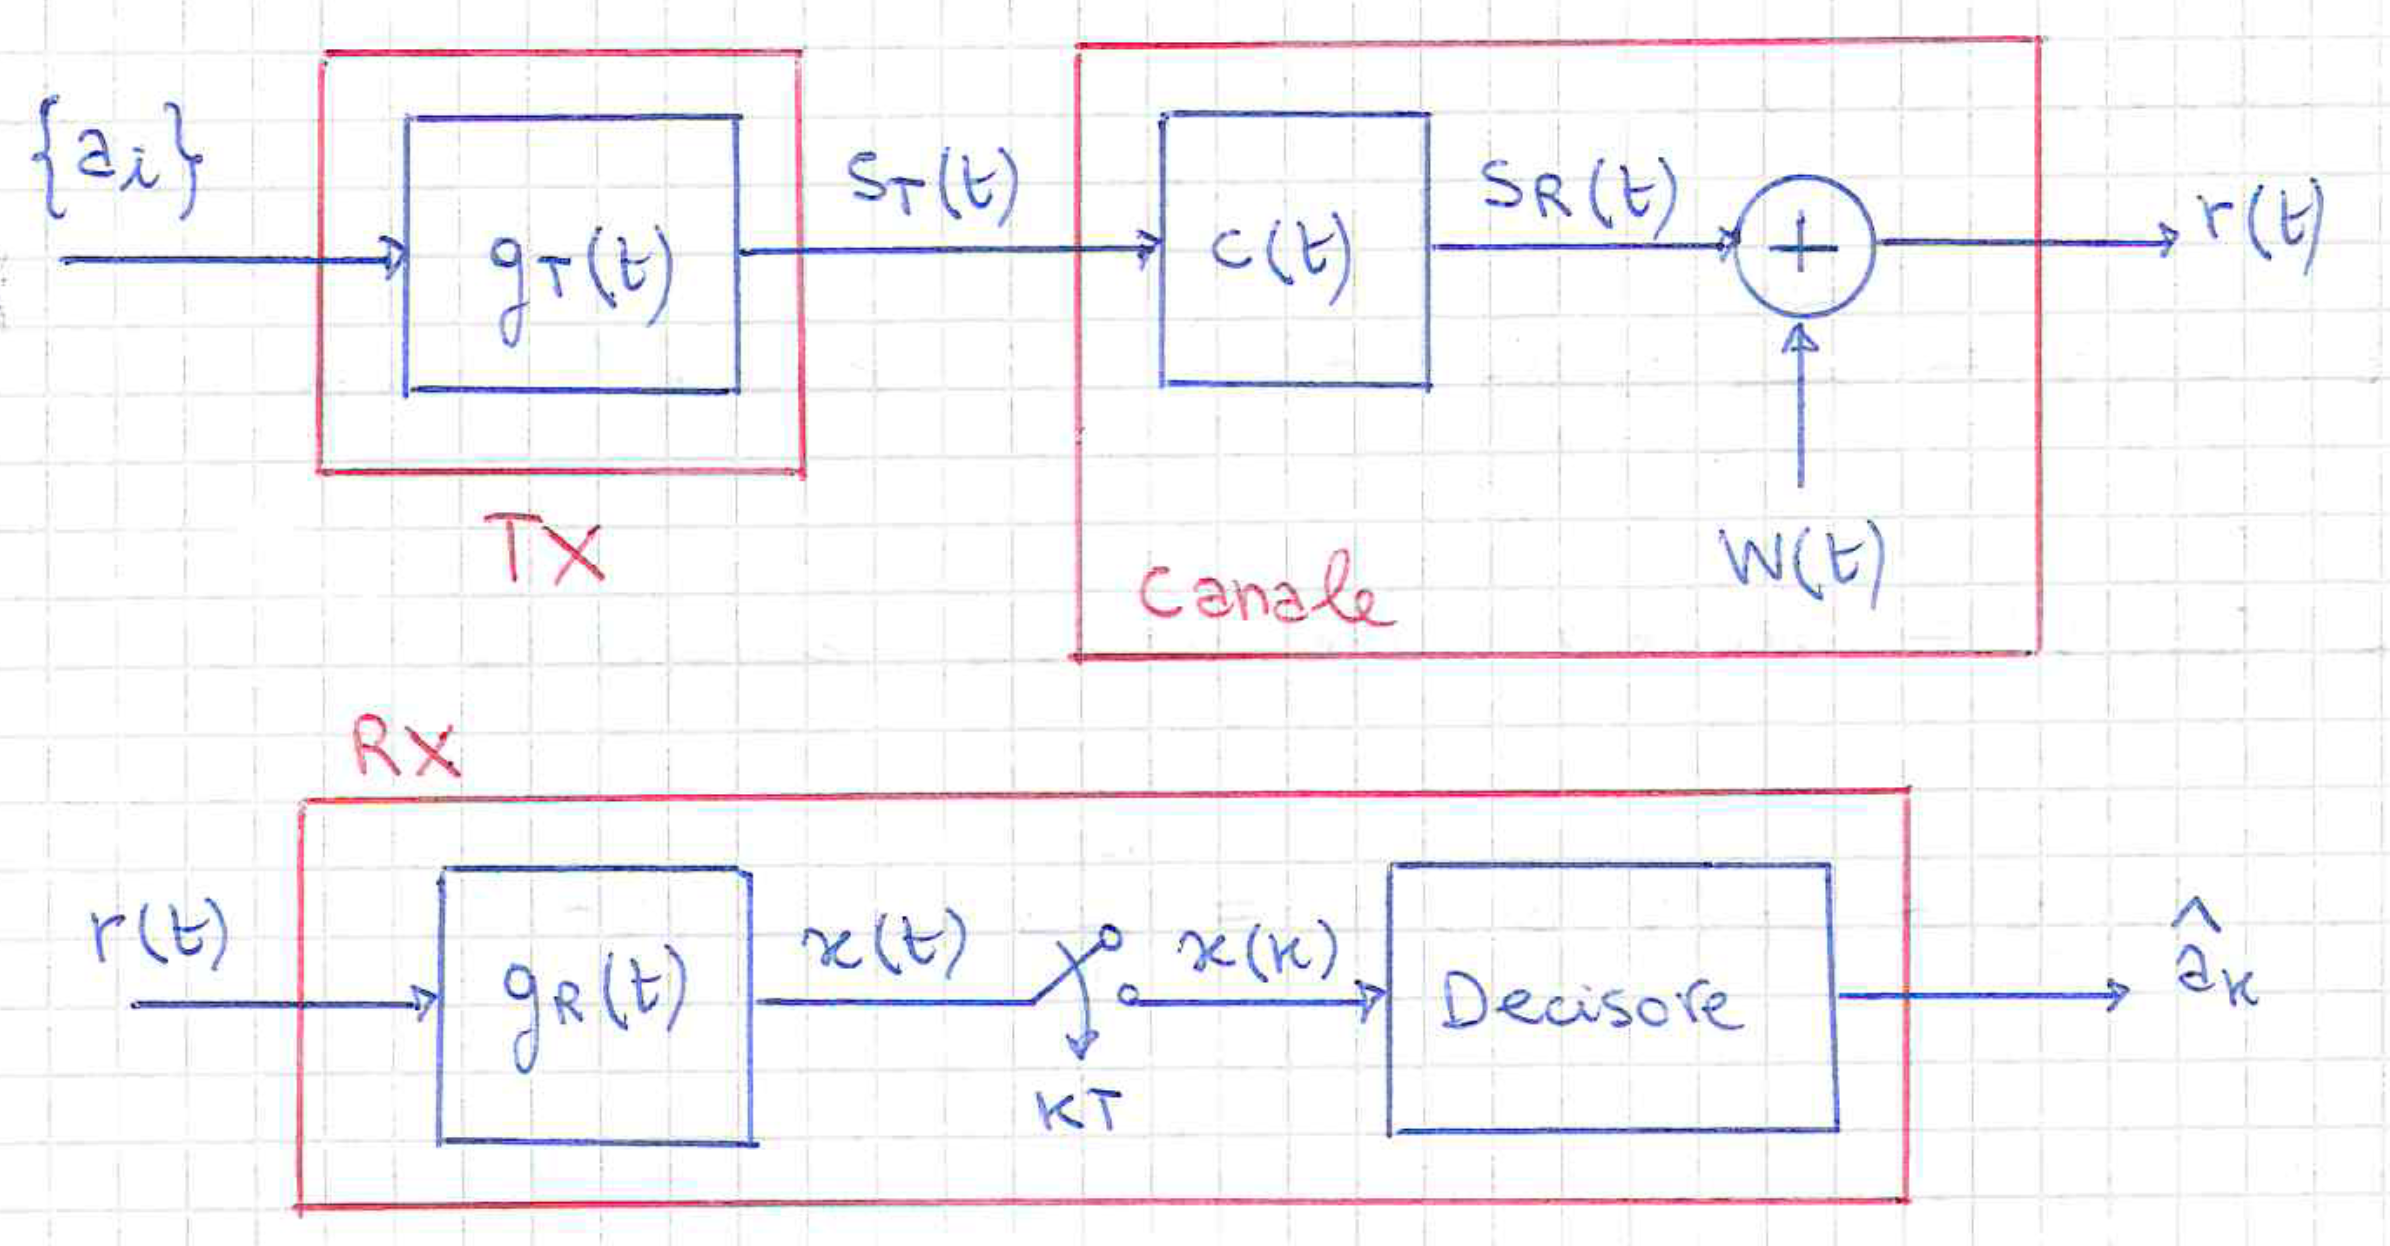
\includegraphics[scale=0.16]{../figures/full_sys.png}
\end{center}

Ciò che facciamo è prendere il segnale dall'etere, mandarlo in ingresso ad un filtro (che chiamiamo $g_R(t)$), e campionarlo ad intervalli $k T_S$, $k \in \mathbb{Z}$. Notiamo che se nel nostro segnale c'è un dato ritardo $\tau$, dovremo campionare ad intervalli $k T_S + \tau$. 

Tratando matematicamente i segnali, abbiamo che a valle del filtro di ricezione $g_R(t)$ abbiamo un segnale convoluto:
$$
x(t) = r(t) \circledast g_R(t) = \sqrt{\beta} S_T(t - \tau) \circledast g_R(t) + w(t) \circledast g_R(t)
$$
Chiamiamo $ w(t) \circledast g_R(t) = n(t) $ per il rumore. Sostituendo la $S_T(t)$, otterremo:
$$
x(t) = \sqrt{\beta} \sum_i a_i g_T ( t - i T_S - \tau) \circledast g_R(t) + h(t)
$$

Combiniamo i filtri di trasmissione e di ricezione in un unico termine $g$:
$$
g(t) = g_T(t) \circledast g_R(t)
$$
per ottenere:
$$
x(t) = \sqrt{\beta} \sum_i a_i g(t - i T_S - \tau) + n(t)
$$

\subsubsection{Rumore}
Parliamo del rumore $n(t)$. Questo sarà dato dal filtraggio di un rumore bianco ($w(t)$), per cui sarà sempre gaussiano, ma a meno che il filtro non sia piatto su tutta la banda, non sarà sempre bianco.
Infatti, la distribuzione di potenza non sarà più per forza piatta:
$$
S_n(f) = S_w(f) | G_R(f) |^2 = \frac{N_0}{2} | G_R(f) |^2
$$
con potenza complessiva:
$$
P_n = \int_{-\infty}^{\infty} S_n(f) \, df = \frac{N_0}{2} E_{g_R}
$$

\subsubsection{Campionamento}
Dopo aver caratterizzato $x(t)$, cioè l'ultimo stadio \textit{analogico} del demodulatore (dove avevamo il segnale filtrato dal mezzo, più il rumore introdotto, filtrati dal filtro di ricezione), campioniamo tale segnale come campionato a intervalli $k T_S + \tau$:
$$
x(k) = x(k T_S + \tau) = \sqrt{\beta} \sum_i a_i g((k - i) T_S) + n(k)
$$
Quest'espressione si semplifica ponendo $m = k - i$, per cui:
$$
x(k) = \sqrt{\beta} \sum_m a_{k - m} g(m T_S) + n(k) = 
\sqrt{\beta} \left( a_k g(0) + \sum_{m \neq 0} a_{k - m} g(m T_S) + \frac{n(k)}{\sqrt{\beta}} \right)
$$

Di questa formula, cio che ci interessa è chiaramente il simbolo $a_k$, a cui sommiamo il rumore $n(k)$ (caricato del guadagno), e il termine:
$$
\mathrm{ISI} = \sum_{m \neq 0} a_{k - m} g(m T_S)
$$
che denominiamo \textbf{ISI} (o IIS, da\textit{Interferenza Inter-Simbolica}), dato dall'errore introdotto dagli altri simboli (interpolati) sul segnale in $k$.

\subsubsection{Dimensionamento dei filtri}
Un'incognita che è rimasta finora, sia nel trasmettitore che nel modulatore, è il dimensionamento dei filtri di trasmissione e di ricezione. Facciamolo adesso, che abbiamo una vista di insieme anche di ciò che accade al ricevitore.

L'obiettivo dell'ottimizzazione sarà senza dubbio quello di annullare l'ISI, che ricordiamo definiamo come:
$$
\mathrm{ISI} = \sum_{m \neq 0} a_{k - m} g(m T_S), \quad g(t) = g_T(t) \circledast g_R(t)
$$
Chiamiamo questa condizione anche \textit{condizione di assenza di interferenza inter-simbolica}.
Imponiamo quindi la nullità:
$$
g(m T_S) = 0, \quad \forall m \neq 0
$$
Buone opzioni per questa $g$ sono la $\mathrm{sinc}$ o ad esempio la $\mathrm{tri}$ su supporto $-T_S$, $T_S$, in quanto hanno picco in $0$ e si annullano per la prima volta in $\pm T_S$. Esprimiamo allora la convoluzione:
$$
g(t) = \int_{-\infty}^\infty g_T(\alpha) g_R(t - \alpha) \, d\alpha, \quad g(m) = \int_{-\infty}^\infty g_T(\alpha) g_R(m T_S - \alpha) \, d\alpha 
$$

Passiamo al dominio frequenziale, prendendo la trasformata discreta:
$$
\overline{G} (f) = \sum_m g(m T_S) e^{-i 2 \pi f m T_S} = \frac{1}{T_S} \sum_k G\left( f - \frac{k}{T_S} \right) = g(0)
$$
Questo significa che imporre $g(0) = \gamma$ con $\gamma$ costante qualsiasi solo per $m = 0$ (e $0$ altrove) equivale a imporre che le immagini in frequenza si sovrappongano, a dare un segnale costante (in dominio frequenziale).

Questo significa che è necessario che la banda del filtro $G$ (chiamiamola $B_G$) sia almeno $\frac{1}{2 T_S}$ (cioè si verifichi sovrapposizione). Il caso $B_G = \frac{1}{2 T_S}$ può funzionare solo se lo spettro di $G$ è una $\mathrm{rect}$. 

\par\smallskip

Se questa condizione è rispettata, quindi, l'espressione per la $x(k)$ diventa molto più semplice:
$$
x(k) = \sqrt{\beta} \left( a_k g(0) + \frac{n(k)}{\sqrt{\beta}} \right)
$$
cioè si può ignorare l'interferenza inter-simbolica. Il rumore di fondo purtroppo rimane.

\subsection{Decisore}
Trascuriamo per adesso come si fa il dimensionamento dei singoli filtri (trasmettitore e ricevitore), e passiamo a discutere come ricaviamo le parole di codice a partire dal segnale campionato:
$$
x(k) = \sqrt{\beta} \left( a_k g(0) + \frac{n(k)}{\sqrt{\beta}} \right) \sim a_k + \frac{n(k)}{\sqrt{\beta} g(0)}
$$

Il componente che si occupa di fare ciò viene detto \textit{decisore} o \textbf{demappatore} (l'opposto del \textit{mappatore}). La strategia è quella di prendere la proporzionalità espressa sopra, ed estrapolarla attraverso un passaggio di normalizzazione:
$$
y(k) = \frac{x(k)}{\sqrt{\beta} g(0)} = a_k + \frac{n(k)}{\sqrt{\beta} g(0)}
$$
che in ipotesi di rumore nullo dà esattamente il simbolo $a_k$.

A questo punto si può pensare di trovare il punto più vicino ad $a_k$ nella costellazione adottata al trasmettitore, e ritrovare la parola di codice mappata a tale simbolo. In verità, la decodifica che vogliamo fare non è a minima distanza, ma a massima verosomiglianza (assunto che i simboli trasmessi siano equiprobabili).

\subsubsection{Trattazione del rumore}
Vediamo cosa accade al rumore nel decisore. Avevamo detto che questo era rappresentato da:
$$
n(k), \quad S_n(f) = \frac{N_0}{2} | G_R(f) |^2
$$
Visto che stiamo effettivamente filtrando un processo gaussiano, il risultato sarà anch'esso un processo gaussiano, di cui ci interesseranno le statistiche del primo e del secondo ordine (valor medio e varianza).
Il valor medio è banale in quanto viene dal valor medio del rumore bianco:
$$
\eta_n = E \{ n(k) \} = 0
$$
mentre la varianza viene dalla potenza del rumore:
$$
\sigma_n^2 = E \{ n^2(k) \} = P_n
$$
in quanto lo spettro del rumore bianco è costante (di per sé varianza infinita), e ciò che conta sono solo i parametri $N_0$ e l'integrale della densità di potenza di $G_R(f)$:
$$
P_n = \frac{N_0}{2} E_{g_R}
$$

\end{document}
